\newpage
\subsection{Sequenzdiagramm}
\subsubsection{Queueing}
Das Queueing Sequenzdiagramm beschreibt den Parallelisierungprozess.
\\
\begin{figure}[H]
	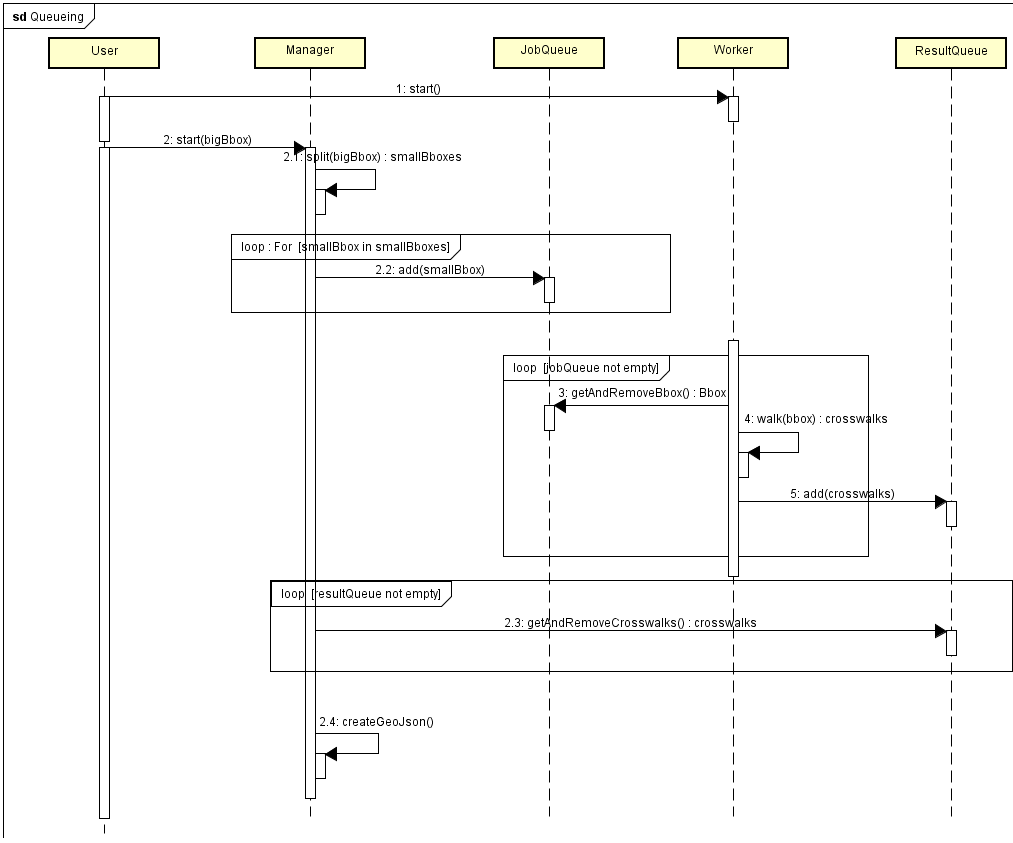
\includegraphics[width=\textwidth]{images/seq_queueing.png}
	\caption{Sequenzdiagramm Queueing}
\end{figure}

\newpage
\subsubsection{Walking}
Das Walking Sequenzdiagramm beschreibt den Ablauf, wie eine Bounding Box von einem Jobworker abgearbeitet wird.
\\
\begin{figure}[H]
	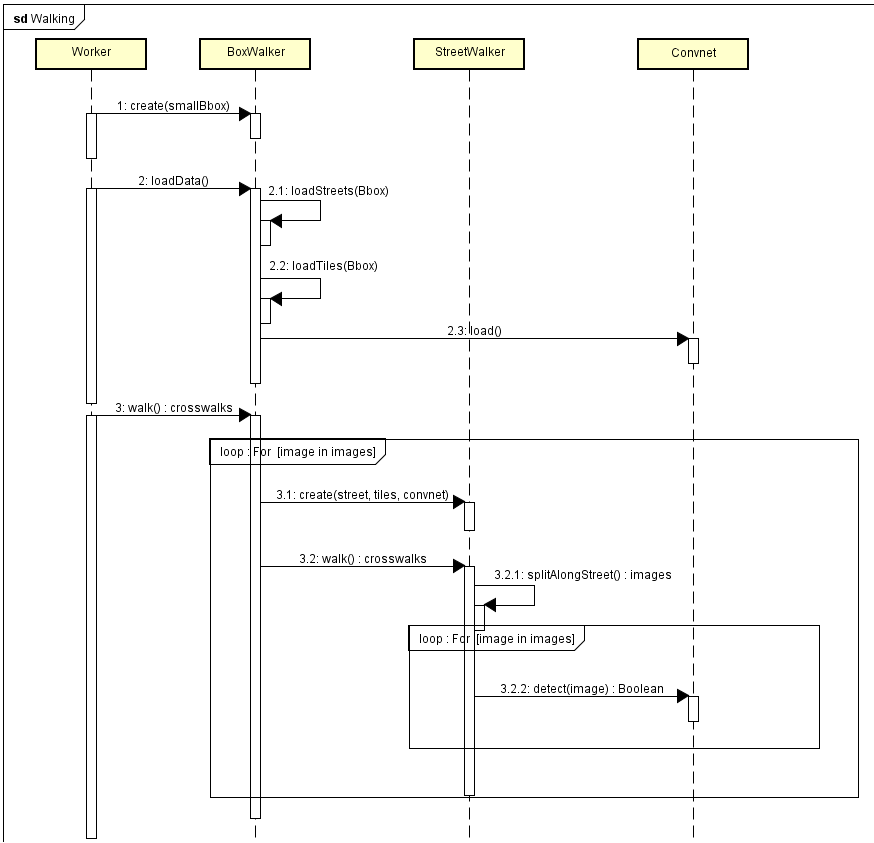
\includegraphics[width=\textwidth]{images/seq_walking.png}
	\caption{Sequenzdiagramm Walking}
\end{figure}
\newpage